\documentclass[a4paper,10pt]{article}
\usepackage[utf8]{inputenc} %Codificacion utf-8
\usepackage{graphicx}
\usepackage{enumerate}
\usepackage{fancyhdr}
\usepackage{hyperref}
\usepackage{tikz}     % graphs!
\usepackage{listings} % code!
\usepackage{multirow} % Required for multirows
\usepackage[spanish, activeacute]{babel} %Definir idioma español
% \usepackage[margin=3cm]{geometry}
\usepackage{cite} % para contraer referencias
\usepackage{url}
\makeatletter
\renewenvironment{thebibliography}[1]
     {\section*{\bibname}% <-- this line was changed from \chapter* to \section*
      \@mkboth{\MakeUppercase\bibname}{\MakeUppercase\bibname}%
      \list{\@biblabel{\@arabic\c@enumiv}}%
           {\settowidth\labelwidth{\@biblabel{#1}}%
            \leftmargin\labelwidth
            \advance\leftmargin\labelsep
            \@openbib@code
            \usecounter{enumiv}%
            \let\p@enumiv\@empty
            \renewcommand\theenumiv{\@arabic\c@enumiv}}%
      \sloppy
      \clubpenalty4000
      \@clubpenalty \clubpenalty
      \widowpenalty4000%
      \sfcode`\.\@m}
     {\def\@noitemerr
       {\@latex@warning{Empty `thebibliography' environment}}%
      \endlist}
\makeatother

\usepackage[nottoc,numbib]{tocbibind}
\setlength{\parskip}{1em}
\setlength{\headheight}{15pt}
\hypersetup{
    colorlinks=true,
    linkcolor=blue,
    filecolor=magenta,
    urlcolor=cyan,
}
\pagestyle{fancy}

\lhead{GEMS}
\rfoot{Página \thepage}
\lfoot{Sistemas inteligentes}
\cfoot{}

\newcommand\tab[1][1cm]{\hspace*{#1}}

\title{GEMS, an Expert Managment System.}
\author{Manuel Alejandro Luque León, 46269831H\\Diego Rodríguez Riera, 15404939E}

\begin{document}

\maketitle
\pagebreak
\tableofcontents
\pagebreak

\section{Descripción del problema}
\paragraph{}El problema propone la creación de un \textbf{sistema experto para la clasificación de minerales}. Para esto se seguirán las líneas expuestas a continuación:

\textit{Dadas las características de un mineral (por ejemplo, forma, color, dureza,...), el sistema debe indicar el nombre de dicho mineral.  El número mínimo de características a considerar debe ser 5, y el número de minerales diferentes que tenga predefinido el sistema debe ser de 25.}
\pagebreak


\section{Análisis del problema}
\paragraph{Cualquier} otro detalle de análisis, diseño e implementación (poniendo énfasis en las técnicas usadas para controlar el razonamiento) que pueda ser de interés.
\pagebreak


\section{Manual de usuario}
\subsection{Cómo usar GEMS}
\paragraph{}El uso del software GEMS es muy simple. Nada más cargarlo en clips con:
\begin{lstlisting}
  (load "GEMS.clp")
\end{lstlisting}
Y ejecutar en la consola de \textit{CLIPS}:
\begin{lstlisting}
  (reset)
  (run)
\end{lstlisting}
Se abrirá la interfaz del menú donde podremos elegir entre las opciones posible introduciendo el número correspondiente y pulsando \textit{intro}.
\begin{figure}[ht]
  \centering
  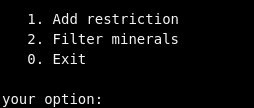
\includegraphics[width=50mm]{./figures/Figure1.png}
\end{figure}

\textbf{\chapter{1. Add restriction}}
\paragraph{}Esta opción del menú permite añadir o modificar las restricciones del filtrado actual. Por defecto al abrir el software no hay ninguna restricción. Si elegimos esta opción, \textit{GEMS} nos mostrará un submenú con las posibles restricciones a aplicar:
\begin{figure}[ht]
  \centering
  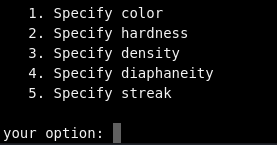
\includegraphics[width=50mm]{./figures/Figure2.png}
\end{figure}

\chapter{1. Specify color}
\setlength{\parskip}{0.5em}
\paragraph{}Permite escoger el color que se usará como filtro. Este color debe ser uno de los siguientes valores: \textit{black, violet, blue, green, yellow, white, pink, red, brown y colorless}.

En caso de introducir uno que no esté en este rango \textit{GEMS} se encargará de pedir que se introduzca uno que sí se encuentre en este rango de valores.

Si se quisiera cambiar el valor del filtro actual bastará con seleccionar esta opción e introducir otro color válido.
\setlength{\parskip}{1em}\\

\chapter{2. Specify hardness}
\setlength{\parskip}{0.5em}
\paragraph{}Permite escoger la dureza medida en \textit{escala de Mohs} que se usará para filtrar los minerales. Por defecto, se mostrarán todos los minerales con un error de 0.3 sobre la dureza introducida por el usuario. Esto se define en el código de \textit{GEMS} a través de la macro \textit{hardnessError}.

Como es conocido, la \textit{escala de Mohs} va del 0 al 10, cualquier número fuera de este rango no será aceptado por \textit{GEMS}.

Al igual que en el apartado anterior, si se quisiera cambiar el valor del filtro actual bastará con seleccionar esta opción e introducir otro valor válido. De aquí en adelante, esto no se mencionará para los demas apartados del submenú ya que todos funcionan igual.
\setlength{\parskip}{1em}\\

\chapter{3. Specify density}
\setlength{\parskip}{0.5em}
\paragraph{}Desde esta opción podremos escoger la densidad medida en \textit{g/cm³} por la que se desean filtrar los minerales. Por defecto, se mostrarán todos los minerales con un error de 0.1 sobre la densidad introducida por el usuario. Esto se define en el código de \textit{GEMS} a través de la macro \textit{densityError}.

\textit{GEMS} aceptará como valor válido para esta propiedad cualquiera número positivo.
\setlength{\parskip}{1em}\\

\chapter{4. Specify diaphaneity}
\setlength{\parskip}{0.5em}
\paragraph{}Permite asignar el valor de transparencia por el que se filtrarán los minerales. Los valores válidos son: \textit{transparent, translucent y opaque}. Se escogerá el valor deseado con el submenú que aparecerá en pantalla.

En caso de introducir un valor no válido, \textit{GEMS} se asegurá de que se introduzca otro valor hasta que se introduzca uno válido.
\setlength{\parskip}{1em}\\

\chapter{5. Specify streak}
\setlength{\parskip}{0.5em}
\paragraph{}Esta opción permite escoger el color de la raya por el que filtrar los minerales. Los valores válidos son los mismos que acepta la opción \textit{1. Specify color}: \textit{black, violet, blue, green, yellow, white, pink, red, brown y colorless}.

En caso de introducir uno que no esté en este rango \textit{GEMS} se encargará de pedir que se introduzca uno que sí se encuentre en este rango de valores.
\setlength{\parskip}{1em}\\

\textbf{\chapter{2. Filter minerals}}
\paragraph{}Al escoger esta opción se imprimirán todos los minerales que concuerden con las restricciones actuales. Si se desea modificar alguna de las restricciones basta con volver a introducir un valor para ella. Para resetear los valores del filtro a por defecto habrá que cerrar y abrir de nuevo el programa.

\textbf{\chapter{0. Exit}}
\paragraph{}Cierra \textit{GEMS} y \textit{CLIPS} volviendo a la terminal del sistema.

\subsection{Base de datos de GEMS}


\pagebreak

\section{Colaboradores}
\paragraph{}Ambos autores hemos trabajado conjuntamente sobre github, Diego Rodríguez Riera se especializó en el diseño y programación del sistema experto y Manuel Alejandro Luque León en la recolecta de información y creación de la base de datos. Finalmente, ambos trabajamos por igual en la creción de la documentación.
\pagebreak

\nocite{*}

\bibliography{biblio.bib}
\bibliographystyle{alpha}
\end{document}
